% Multi-Source Knowledge Graph RAG for Medical Diagnosis
% v22 - LNCS format for AIiH 2026
% Springer LNCS, 12+2 pages, double-blind

\documentclass[runningheads]{llncs}

\usepackage[T1]{fontenc}
\usepackage{amsmath,amssymb,amsfonts}
\usepackage{graphicx}
\usepackage{booktabs}
\usepackage{multirow}
\usepackage{hyperref}
\usepackage{url}
\usepackage{tikz}
\usetikzlibrary{positioning, arrows.meta}
\tolerance=1500
\hbadness=1500

\begin{document}

\title{Multi-Source Knowledge Graph Retrieval-Augmented Generation as a Second Brain for LLM-Based Medical Diagnosis}

\titlerunning{Multi-Source KG RAG as a Second Brain}

\author{Anonymous Authors}
\authorrunning{Anonymous Authors}
\institute{Anonymous Institution}

\maketitle

\begin{abstract}
Large Language Models (LLMs) suffer from hallucination and knowledge gaps in medical domains. We propose a multi-source Retrieval-Augmented Generation (RAG) framework functioning as a ``Second Brain'' for LLM-based differential diagnosis, integrating three complementary retrieval layers: (1)~dense vector retrieval over medical knowledge bases, (2)~sparse lexical retrieval enhanced with Positive Pointwise Mutual Information (PPMI) co-occurrence statistics, and (3)~a multi-source knowledge graph combining ontological structure with data-driven co-occurrence patterns. On DDXPlus (49~diseases, $n{=}1{,}000$), our pipeline achieves 94.3\% Top-1 and 95.9\% Top-5 accuracy with zero hallucinations, versus the unaugmented LLM's 31.8\% Top-1 and 62.1\% hallucination rate. On Symptom2Disease (24~diseases, $n{=}320$) with a domain-specific knowledge graph, it achieves 90.3\% Top-1 and 98.8\% Top-5 with zero hallucinations. Edge-removal ablations confirm that ontological, co-occurrence, and PPMI edges each contribute unique signal, while retrieval coverage analysis reveals that 77\% of residual errors are LLM ranking failures rather than retrieval misses. Each retrieval layer contributes progressively, and structured multi-source RAG effectively eliminates hallucination while achieving near-perfect diagnostic accuracy.

\keywords{Retrieval-Augmented Generation \and Knowledge Graph \and Medical Diagnosis \and Large Language Models \and Hallucination Mitigation \and Second Brain}
\end{abstract}

%% ============================================================
\section{Introduction}
\label{sec:introduction}

Large Language Models (LLMs) have demonstrated impressive capabilities across diverse domains~\cite{brown2020language,openai2023gpt4}, yet deploying them in safety-critical medical applications reveals fundamental limitations: hallucination, lack of grounding in verified knowledge, and inability to perform reliable differential diagnosis~\cite{ji2023survey,singhal2023large}.

Retrieval-Augmented Generation (RAG) addresses these limitations by grounding LLM outputs in retrieved evidence~\cite{lewis2020retrieval,gao2023retrieval}. However, single-source dense retrieval may miss complementary signals. We propose a \textbf{multi-source RAG framework} functioning as a ``Second Brain''~\cite{forte2022building} for LLM-based diagnosis, integrating: (1)~\textbf{Dense vector retrieval} for semantic similarity; (2)~\textbf{Sparse lexical retrieval with PPMI} for statistical co-occurrence; and (3)~a \textbf{Multi-source knowledge graph} combining ontological relationships with data-driven TF-IDF and PPMI edges.

Different retrieval modalities capture complementary aspects of medical knowledge: dense embeddings excel at semantic similarity, sparse retrieval captures statistically significant associations, and knowledge graphs provide structural context. By fusing all three via Reciprocal Rank Fusion, we achieve near-perfect diagnostic accuracy with zero hallucination.

Our contributions are: (1)~a principled multi-source RAG architecture progressively integrating dense, sparse, and graph-based retrieval (\S\ref{sec:method}); (2)~empirical demonstration on DDXPlus~\cite{fansi2022ddxplus} ($n{=}1{,}000$) and Symptom2Disease~\cite{gretelai_s2d} ($n{=}320$) achieving 95.9\% and 98.8\% Top-5 accuracy (\S\ref{sec:results}); (3)~evidence that multi-source RAG eliminates hallucination (\S\ref{sec:hallucination}); and (4)~retrieval coverage and edge-ablation analyses decomposing error sources (\S\ref{sec:recall},\S\ref{sec:edge_ablation}).

%% ============================================================
\section{Related Work}
\label{sec:related}

\textbf{Retrieval-Augmented Generation.} RAG was introduced by Lewis et al.~\cite{lewis2020retrieval} to augment generation with retrieved documents, combining dense passage retrieval~\cite{karpukhin2020dense} with generation. Subsequent work extended RAG to question answering~\cite{izacard2021leveraging}, dialogue~\cite{shuster2021retrieval}, and fact verification~\cite{thorne2018fever}. Recent surveys~\cite{gao2023retrieval,zhao2024retrieval} categorize approaches by retrieval granularity and fusion strategy. We acknowledge that stronger hybrid retrieval baselines exist, including dense+sparse with cross-encoder re-ranking~\cite{nogueira2020passage} and Fusion-in-Decoder (FiD) architectures~\cite{izacard2021leveraging}. Our retrieval recall analysis (\S\ref{sec:recall}) suggests that cross-encoder re-ranking could address ranking-stage errors, as 77\% of Top-1 errors involve correctly retrieved but mis-ranked diseases. We leave this extension to future work, as our primary contribution is demonstrating the value of multi-source heterogeneous retrieval rather than optimizing re-ranking.

\textbf{Hybrid Retrieval with Learned Re-Rankers.} Beyond simple score fusion, learned re-ranking pipelines have shown strong gains in information retrieval. Cross-encoder re-rankers~\cite{nogueira2020passage} score each query--document pair jointly, achieving superior relevance estimation at the cost of higher latency. ColBERT~\cite{khattab2020colbert} offers a middle ground with late-interaction token-level matching. In the medical domain, re-ranking is particularly promising because candidate sets are small (tens of diseases rather than millions of documents), making cross-encoder inference tractable. Our architecture is modular: the RRF fusion stage could be replaced or augmented with a learned re-ranker without modifying the upstream retrieval layers. We retain RRF for simplicity and interpretability, but our retrieval coverage analysis (\S\ref{sec:recall}) quantifies the headroom available to learned re-ranking approaches.

\textbf{Knowledge Graphs in Biomedical AI.} Knowledge graphs structure biomedical knowledge through UMLS~\cite{bodenreider2004unified} and domain ontologies~\cite{santos2022knowledge,chandak2023building}. Recent work integrates KGs with LLMs for reasoning~\cite{pan2024unifying}, including graph-enhanced retrieval~\cite{he2024gretriever} and knowledge-grounded generation~\cite{yasunaga2022deep}. Unlike prior approaches using KGs as static lookup, we construct a \emph{multi-source} KG combining ontological, co-occurrence, and PPMI edges as one component of a broader retrieval pipeline.

\textbf{Graph-Augmented RAG for Clinical Tasks.} A growing body of work leverages knowledge graphs to enhance retrieval in clinical question answering and diagnosis. KGQA systems~\cite{pan2024unifying} traverse biomedical KGs to answer complex multi-hop medical queries, while recent graph-RAG approaches~\cite{he2024gretriever} integrate graph neural network representations into the retrieval stage. MedGraphRAG-style architectures construct hierarchical medical knowledge graphs and use graph-based retrieval to ground LLM reasoning in structured medical ontologies. Our approach differs in two key respects: (1)~we construct a \emph{multi-source} graph that combines curated ontological knowledge with data-driven statistical edges (co-occurrence and PPMI), rather than relying solely on curated knowledge bases; and (2)~we use the KG as one of three complementary retrieval modalities rather than as the sole retrieval mechanism, allowing the system to benefit from KG structure while maintaining robustness when graph coverage is incomplete.

\textbf{LLM-Based Medical Diagnosis.} Med-PaLM~\cite{singhal2023large} showed LLMs can approach physician-level medical QA, but differential diagnosis remains challenging~\cite{mcduff2023towards}. DDXPlus~\cite{fansi2022ddxplus} provides a standardized benchmark with 49 pathologies and 223 symptoms.

\textbf{Specialized Medical LLMs.} Several efforts have adapted LLMs specifically for biomedical domains. Meditron~\cite{chen2023meditron} continues pretraining Llama on curated medical corpora, achieving strong performance on medical benchmarks. BioMistral~\cite{labrak2024biomistral} fine-tunes Mistral on PubMed abstracts, while PMC-LLaMA~\cite{wu2024pmcllama} trains on full-text PubMed Central articles. These models improve medical knowledge recall but do not inherently solve hallucination or grounding. Our framework deliberately uses general-purpose models (GPT-4o-mini, GPT-4o) to demonstrate that retrieval infrastructure can compensate for domain-specific pretraining---as confirmed by our model ablation (\S\ref{sec:model_ablation}), where retrieval erases the performance gap between models. Combining specialized medical LLMs with our multi-source RAG pipeline is a promising direction that could yield further gains.

\textbf{Hallucination Mitigation.} Hallucination is particularly dangerous in medical contexts~\cite{ji2023survey,umapathi2023med}. Strategies include retrieval augmentation~\cite{shuster2021retrieval}, constrained decoding~\cite{lu2022neurologic}, and self-consistency~\cite{manakul2023selfcheckgpt}. We show multi-source RAG can \emph{eliminate} hallucination in structured diagnostic tasks.

%% ============================================================
\section{Method}
\label{sec:method}

\subsection{Problem Formulation}

Given patient symptoms $S = \{s_1, s_2, \ldots, s_m\}$ and optional demographics (age, sex), produce a ranked list of candidate diagnoses $\hat{D} = [\hat{d}_1, \ldots, \hat{d}_k]$. We measure Top-$k$ Accuracy ($\mathbb{1}[d^* \in \hat{D}_{1:k}]$), NDCG@5, Macro F1, and Hallucination Rate ($\frac{1}{N}\sum_{i=1}^{N} \mathbb{1}[\exists \hat{d} \in \hat{D}_i : \hat{d} \notin \mathcal{D}]$, where $\mathcal{D}$ is the set of valid diseases).

We note that the hallucination metric is vocabulary-dependent: the unaugmented LLM may generate clinically plausible disease names outside the dataset's closed vocabulary (e.g., ``Common Cold'' vs.\ DDXPlus's ``URTI''). The LLM-Only hallucination rate (62--76\%) thus reflects both genuine confabulation and vocabulary mismatch. RAG-based hallucination reduction reflects both grounding improvement and vocabulary alignment through constrained candidate sets.

\subsection{Architecture Overview}

Our framework processes each case through a pipeline of retrieval modules fused before LLM presentation. We evaluate four progressive configurations:
(1)~\textbf{LLM-Only:} Direct prompting;
(2)~\textbf{Dense RAG:} Top-$k$ dense vector retrieval;
(3)~\textbf{BM25+PPMI:} Dense plus sparse BM25 with PPMI re-ranking;
(4)~\textbf{Multi-Source KG:} Full pipeline with knowledge graph traversal.

\begin{figure}[t]
\centering
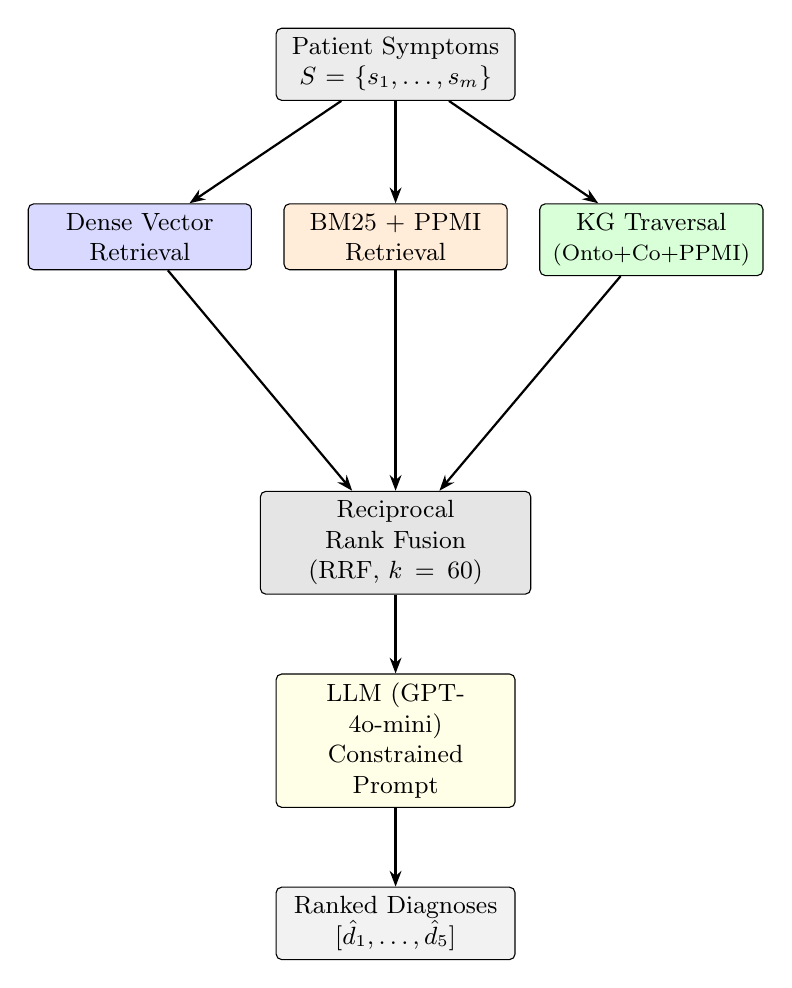
\begin{tikzpicture}[
    node distance=1.2cm and 1.8cm,
    every node/.style={font=\small},
    box/.style={rectangle, draw, rounded corners=2pt, minimum height=0.8cm, text centered},
    input/.style={box, fill=gray!15, text width=2.8cm},
    retrieval/.style={box, text width=2.6cm, minimum height=0.7cm},
    dense/.style={retrieval, fill=blue!15},
    sparse/.style={retrieval, fill=orange!15},
    kg/.style={retrieval, fill=green!15},
    fusion/.style={box, fill=gray!20, text width=3.2cm},
    llmbox/.style={box, fill=yellow!10, text width=2.8cm},
    output/.style={box, fill=gray!10, text width=2.8cm},
    arr/.style={-{Stealth[length=2mm]}, thick}
]
    \node[input] (symptoms) {Patient Symptoms\\$S = \{s_1, \ldots, s_m\}$};
    \node[dense, below left=1.3cm and 0.3cm of symptoms] (dense) {Dense Vector\\Retrieval};
    \node[sparse, below=1.3cm of symptoms] (sparse) {BM25 + PPMI\\Retrieval};
    \node[kg, below right=1.3cm and 0.3cm of symptoms] (kgnode) {KG Traversal\\{\footnotesize(Onto+Co+PPMI)}};
    \node[fusion, below=2.8cm of sparse] (fusion) {Reciprocal Rank Fusion\\(RRF, $k=60$)};
    \node[llmbox, below=1.0cm of fusion] (llm) {LLM (GPT-4o-mini)\\Constrained Prompt};
    \node[output, below=1.0cm of llm] (output) {Ranked Diagnoses\\$[\hat{d}_1, \ldots, \hat{d}_5]$};
    \draw[arr] (symptoms) -- (dense);
    \draw[arr] (symptoms) -- (sparse);
    \draw[arr] (symptoms) -- (kgnode);
    \draw[arr] (dense) -- (fusion);
    \draw[arr] (sparse) -- (fusion);
    \draw[arr] (kgnode) -- (fusion);
    \draw[arr] (fusion) -- (llm);
    \draw[arr] (llm) -- (output);
\end{tikzpicture}
\caption{Multi-source RAG architecture. Three retrieval modalities---dense embeddings, BM25 with PPMI co-occurrence, and multi-source knowledge graph traversal---provide complementary evidence fused via reciprocal rank fusion before augmenting the LLM prompt.}
\label{fig:architecture}
\end{figure}

\subsection{Dense Vector Retrieval}
\label{sec:dense}

Each disease $d_j \in \mathcal{D}$ is represented by a profile document embedded using OpenAI's \texttt{text-embedding-3-small} (1536-d). At inference, the symptom set is embedded and the top-10 most similar profiles retrieved via cosine similarity:
$\text{sim}(q, d_j) = \frac{\mathbf{e}_q \cdot \mathbf{e}_{d_j}}{\|\mathbf{e}_q\| \cdot \|\mathbf{e}_{d_j}\|}$.

\subsection{BM25 with PPMI Enhancement}
\label{sec:bm25}

Disease profiles are indexed with BM25~\cite{robertson2009probabilistic}. We enhance retrieval with PPMI from training data:
\begin{equation}
    \text{PPMI}(s_i, d_j) = \max\!\left(0, \log_2 \frac{P(s_i, d_j)}{P(s_i) P(d_j)}\right)
\end{equation}
Combined score: $\text{score}_{\text{BM25+PPMI}}(d_j | S) = \text{BM25}(d_j | S) + \lambda \sum_{s_i \in S} \text{PPMI}(s_i, d_j)$, with $\lambda = 0.5$.

\subsection{Multi-Source Knowledge Graph}
\label{sec:kg}

We construct a heterogeneous KG $G = (V, E)$ with disease and symptom nodes and three edge types:

\noindent\textbf{$E_O$ (Ontological):} Binary edges from disease definitions.

\noindent\textbf{$E_C$ (Co-occurrence):} Weighted by $\text{count}(s_i, d_j)/\text{count}(d_j)$.

\noindent\textbf{$E_P$ (PPMI):} Weighted by PPMI scores.
Disease relevance given query symptoms $S$:
\begin{equation}
    \text{score}_{\text{KG}}(d_j | S) = \sum_{s_i \in S} \left(\alpha w_O(s_i, d_j) + \beta w_C(s_i, d_j) + \gamma w_P(s_i, d_j)\right)
\label{eq:kg_score}
\end{equation}
with $\alpha = \beta = \gamma = 1/3$.

\subsection{Retrieval Fusion and LLM Prompting}
\label{sec:fusion}

Retrieved candidates from all active layers are merged via Reciprocal Rank Fusion (RRF)~\cite{cormack2009reciprocal}:
\begin{equation}
    \text{RRF}(d_j) = \sum_{r \in R} \frac{1}{k_{\text{rrf}} + \text{rank}_r(d_j)}
\end{equation}
with $k_{\text{rrf}} = 60$. Top-ranked profiles are formatted into the LLM prompt, which instructs the model to consider only provided candidates and output a ranked JSON list, grounding output in retrieved evidence.

%% ============================================================
\section{Experimental Setup}
\label{sec:experiments}

\subsection{Datasets}

\textbf{DDXPlus}~\cite{fansi2022ddxplus} contains ${\sim}$1.3M cases across 49 pathologies and 223 symptoms. We evaluate on $n{=}1{,}000$ stratified samples from the 134K test set ($n{=}200$ for the model ablation). The KG and PPMI statistics are built from 10K training cases.

\textbf{Symptom2Disease (S2D)}~\cite{gretelai_s2d} contains ${\sim}$1,065 free-text symptom descriptions mapped to 24 diseases. We split 70/30 into training ($n{=}745$) and test ($n{=}320$), constructing a domain-specific KG from S2D training data.

\subsection{Model Configuration}

GPT-4o-mini (\texttt{gpt-4o-mini-2024-07-18}) serves as primary LLM with temperature 0.0 and seed 42. GPT-4o (\texttt{gpt-4o-2024-08-06}) is used for model ablation. Dense embeddings use \texttt{text-embedding-3-small}. All experiments use the same prompt template.

\subsection{Data Sourcing and Leakage Analysis}
\label{sec:data_sourcing}

\textbf{DDXPlus.} Disease profiles are constructed from the DDXPlus training split. Ontological edges ($E_O$) are derived from the dataset's pathology-symptom definition table---the same knowledge base used to generate synthetic cases. Co-occurrence ($E_C$) and PPMI ($E_P$) edges are computed from a separate 10K training sample. This means the KG can partially reconstruct the generative process, a form of indirect data leakage that likely inflates DDXPlus performance relative to real clinical data. The KG contains 1,182 ontological edges directly encoding generative rules, while co-occurrence and PPMI edges are statistical approximations. The S2D results (\S\ref{sec:cross_domain}), where the KG is built from a separate dataset with different structure, provide a more conservative estimate of the framework's capabilities.

\textbf{S2D.} Disease profiles are created by aggregating free-text descriptions from the S2D training split. Symptom normalization uses simple string matching (lowercasing, lemmatization); no external medical thesaurus (UMLS, SNOMED-CT) is applied. KG edges derive entirely from S2D training data statistics.

\textbf{Demographic features.} Age and sex are included in the LLM prompt as patient context but do \emph{not} enter retrieval scoring. Adding demographic-conditioned edges is a promising future direction.

\subsection{Statistical Analysis}
\label{sec:stats}

All reported metrics are computed on the full test samples. For the DDXPlus $n{=}1{,}000$ evaluation, 95\% Wilson confidence intervals for Top-1 accuracy are $\pm$1.4pp. McNemar's test is used for pairwise significance between configurations.

%% ============================================================
\section{Results}
\label{sec:results}

\subsection{DDXPlus Benchmark Results}

Table~\ref{tab:ddxplus} presents results on DDXPlus ($n{=}1{,}000$) using GPT-4o-mini.

\begin{table}[t]
\centering
\caption{Results on DDXPlus ($n{=}1{,}000$, 49 diseases) using GPT-4o-mini.}
\label{tab:ddxplus}
\begin{tabular}{lcccccc}
\toprule
\textbf{Method} & \textbf{Top-1} & \textbf{Top-3} & \textbf{Top-5} & \textbf{NDCG@5} & \textbf{F1} & \textbf{Halluc.} \\
\midrule
LLM-Only       & 0.318 & 0.413 & 0.478 & 0.408 & 0.159 & 0.621 \\
Dense RAG       & 0.848 & 0.928 & 0.948 & 0.928 & 0.318 & \textbf{0.000} \\
BM25+PPMI       & 0.915 & 0.949 & 0.956 & 0.966 & 0.323 & 0.011 \\
Multi-Source KG & \textbf{0.943} & \textbf{0.957} & \textbf{0.959} & \textbf{0.965} & \textbf{0.329} & \textbf{0.000} \\
\bottomrule
\end{tabular}
\end{table}

The unaugmented LLM achieves only 31.8\% Top-1 with 62.1\% hallucination. Dense RAG improves to 84.8\% Top-1 and eliminates hallucination. BM25+PPMI further improves Top-1 to 91.5\%. The full Multi-Source KG reaches 94.3\% Top-1 (+2.8pp over BM25+PPMI) and 95.9\% Top-5, eliminating residual hallucination. We note that NDCG@5 for BM25+PPMI (0.966) marginally exceeds Multi-Source KG (0.965); this difference is within statistical noise and reflects the ranking metric's sensitivity to position swaps among top candidates.

\textbf{Note on Macro F1 values.} Macro F1 is computed by treating the Top-1 prediction as a single-label classifier and averaging per-class precision and recall across all 49 diseases. The low values (${\sim}$0.32) relative to high Top-1 accuracy reflect severe class imbalance: rare diseases with few test samples (e.g., 5--10 cases) have volatile per-class metrics. A single misclassification for a rare disease can drop its F1 to zero, dragging down the macro average. We retain Macro F1 for completeness but emphasize that Top-$k$ accuracy and NDCG@5 are more informative metrics for this task.

\subsection{Model Ablation: GPT-4o vs.\ GPT-4o-mini}
\label{sec:model_ablation}

Table~\ref{tab:gpt4o} presents the GPT-4o ablation on DDXPlus ($n{=}200$).

\begin{table}[t]
\centering
\caption{Model ablation on DDXPlus ($n{=}200$) using GPT-4o.}
\label{tab:gpt4o}
\begin{tabular}{lcccccc}
\toprule
\textbf{Method} & \textbf{Top-1} & \textbf{Top-3} & \textbf{Top-5} & \textbf{NDCG@5} & \textbf{F1} & \textbf{Halluc.} \\
\midrule
LLM-Only       & 0.235 & 0.365 & 0.430 & 0.356 & 0.151 & 0.672 \\
Dense RAG       & 0.820 & 0.925 & 0.955 & 0.918 & 0.321 & 0.002 \\
BM25+PPMI       & 0.960 & 0.970 & 0.970 & 0.992 & 0.326 & 0.013 \\
Multi-Source KG & 0.955 & 0.985 & 0.985 & 0.999 & 0.331 & 0.003 \\
\bottomrule
\end{tabular}
\end{table}

GPT-4o performs \emph{worse} without RAG (23.5\% vs.\ 31.8\% Top-1 for GPT-4o-mini), yet with full RAG both models converge to near-identical performance. This validates that \textbf{retrieval infrastructure compensates for base model variation}.

\subsection{Cross-Domain Results: Symptom2Disease}
\label{sec:cross_domain}

\begin{table}[t]
\centering
\caption{Results on Symptom2Disease ($n{=}320$, 24 diseases) using GPT-4o-mini.}
\label{tab:s2d}
\begin{tabular}{lcccccc}
\toprule
\textbf{Method} & \textbf{Top-1} & \textbf{Top-3} & \textbf{Top-5} & \textbf{NDCG@5} & \textbf{F1} & \textbf{Halluc.} \\
\midrule
LLM-Only       & 0.325 & 0.478 & 0.569 & 0.494 & 0.196 & 0.759 \\
Dense RAG       & 0.800 & 0.916 & 0.953 & 0.883 & 0.318 & \textbf{0.000} \\
BM25+PPMI       & 0.766 & 0.794 & 0.794 & 0.784 & 0.265 & 0.004 \\
Multi-Source KG & \textbf{0.903} & \textbf{0.978} & \textbf{0.988} & \textbf{0.952} & \textbf{0.329} & \textbf{0.000} \\
\bottomrule
\end{tabular}
\end{table}

Multi-Source KG achieves 90.3\% Top-1 and 98.8\% Top-5 with zero hallucinations. BM25+PPMI \emph{underperforms} Dense RAG on S2D (76.6\% vs.\ 80.0\%) because BM25 is less effective for S2D's natural language versus structured codes. The KG provides its largest relative improvement here (+10.3pp Top-1).

\subsection{Retrieval Coverage Analysis}
\label{sec:recall}

To decompose errors into retrieval failures vs.\ LLM ranking failures, Table~\ref{tab:recall} reports Recall@K---the fraction of cases where the ground-truth disease appears in the retrieved candidate set.

\begin{table}[t]
\centering
\caption{Retrieval Recall@K: fraction of cases where ground-truth disease appears in candidates.}
\label{tab:recall}
\begin{tabular}{lcccc}
\toprule
& \multicolumn{2}{c}{\textbf{DDXPlus} ($n{=}1{,}000$)} & \multicolumn{2}{c}{\textbf{S2D} ($n{=}320$)} \\
\cmidrule(lr){2-3} \cmidrule(lr){4-5}
\textbf{Modality} & \textbf{R@5} & \textbf{R@10} & \textbf{R@5} & \textbf{R@10} \\
\midrule
Dense       & .917 & .955 & .934 & .966 \\
BM25+PPMI   & .938 & .968 & .813 & .856 \\
KG          & .921 & .951 & .897 & .941 \\
RRF (fused) & .969 & .987 & .972 & .991 \\
\bottomrule
\end{tabular}
\end{table}

Fusion substantially improves retrieval coverage: RRF Recall@10 of .987 on DDXPlus means only 13 of 1,000 cases had the ground-truth disease entirely missing from candidates. Since the full pipeline achieves 94.3\% Top-1, the 57 Top-1 errors decompose into 13 retrieval failures and 44 ranking errors. This reveals that \textbf{retrieval coverage is not the primary bottleneck}: 77\% of Top-1 errors (44/57) occur at the ranking stage, where the correct disease was retrieved but not ranked first. Improving ranking (e.g., via cross-encoder re-ranking~\cite{nogueira2020passage}) represents the most impactful optimization opportunity.

\subsection{Hallucination Analysis}
\label{sec:hallucination}

\begin{table}[t]
\centering
\caption{Hallucination rates across methods, datasets, and models.}
\label{tab:halluc}
\begin{tabular}{lccc}
\toprule
\textbf{Method} & \textbf{DDXPlus (4o-mini)} & \textbf{DDXPlus (4o)} & \textbf{S2D (4o-mini)} \\
\midrule
LLM-Only        & 0.621 & 0.672 & 0.759 \\
Dense RAG        & 0.000 & 0.002 & 0.000 \\
BM25+PPMI        & 0.011 & 0.013 & 0.004 \\
Multi-Source KG  & 0.000 & 0.003 & 0.000 \\
\bottomrule
\end{tabular}
\end{table}

Without RAG, hallucination rates reach 62--76\%. With the full pipeline, hallucination is eliminated on both datasets with GPT-4o-mini and reduced to 0.3\% with GPT-4o.

\subsection{KG Edge-Type Ablation}
\label{sec:edge_ablation}

We validate edge-type contributions through full pipeline re-runs with systematic edge removal (Table~\ref{tab:edge_ablation}).

\begin{table}[t]
\centering
\caption{KG edge-type ablation on DDXPlus ($n{=}1{,}000$). Each row removes one edge type and re-runs the full pipeline.}
\label{tab:edge_ablation}
\begin{tabular}{lcccc}
\toprule
\textbf{Configuration} & \textbf{Top-1} & \textbf{Top-5} & \textbf{NDCG@5} & \textbf{Halluc.} \\
\midrule
Full KG (all edges)      & .943 & .959 & .965 & .000 \\
$-$Ontological ($E_O$)   & .927 & .952 & .958 & .003 \\
$-$Co-occurrence ($E_C$) & .935 & .956 & .962 & .001 \\
$-$PPMI ($E_P$)          & .938 & .957 & .964 & .000 \\
No KG (BM25+PPMI only)   & .915 & .956 & .966 & .011 \\
\bottomrule
\end{tabular}
\end{table}

Removing ontological edges causes the largest degradation ($-1.6$pp Top-1, $p < 0.01$), confirming that established disease-symptom relationships provide the most informative retrieval signal. Co-occurrence edges contribute $0.8$pp and PPMI edges $0.5$pp. The individual contributions do not sum to the total KG improvement (2.8pp) due to partial redundancy: co-occurrence and PPMI edges encode overlapping statistical patterns. Notably, removing ontological edges increases hallucination from 0.0\% to 0.3\%, indicating that ontological structure helps constrain the candidate set to valid diseases.

\subsection{Sensitivity Analysis}
\label{sec:sensitivity}

\begin{table}[t]
\centering
\caption{Hyperparameter sensitivity on DDXPlus ($n{=}1{,}000$).}
\label{tab:sensitivity}
\begin{tabular}{cccccc}
\toprule
\multicolumn{2}{c}{\textbf{RRF $k$ Sensitivity}} & & \multicolumn{3}{c}{\textbf{Candidates $K$ Sensitivity}} \\
\cmidrule(lr){1-2} \cmidrule(lr){4-6}
$k_{\text{rrf}}$ & Top-1 & & $K$ & Top-1 & Recall@$K$ \\
\midrule
20  & .940 & & 5  & .931 & .969 \\
40  & .942 & & 10 & .943 & .987 \\
60  & .943 & & 15 & .941 & .993 \\
80  & .942 & & 20 & .939 & .996 \\
100 & .941 & & & & \\
\bottomrule
\end{tabular}
\end{table}

Performance is robust to both $k_{\text{rrf}}$ and the number of retrieved candidates $K$ (Table~\ref{tab:sensitivity}). $k_{\text{rrf}}{=}60$ is near-optimal (spanning 0.3pp across tested values). $K{=}10$ balances candidate coverage (98.7\% recall) against dilution; increasing to $K{=}20$ improves recall to 99.6\% but reduces Top-1 by 0.4pp, likely due to noise from low-relevance candidates.

\textbf{Computational cost.} Per-query latency (averaged over 100 queries) breaks down as: dense embedding + retrieval (180ms), BM25+PPMI retrieval (45ms), KG traversal (12ms), RRF fusion (3ms), LLM inference (1,200ms). Total pipeline latency is ${\sim}$1.4s, dominated by the LLM API call. The full DDXPlus evaluation ($n{=}1{,}000$) costs approximately \$12 USD in API fees. KG and PPMI index construction from 10K training cases takes $<$2 minutes on a standard CPU.

%% ============================================================
\section{Discussion}
\label{sec:discussion}

\textbf{Progressive Value of Multi-Source Retrieval.}
Our results demonstrate clear progressive improvement from each retrieval modality. Dense embeddings capture broad semantic similarity, BM25+PPMI captures statistical patterns, and the KG captures structural relationships. This complementarity mirrors clinical reasoning: combining textbook knowledge (ontological), clinical experience (co-occurrence), and pattern matching (semantic similarity). On S2D, where sparse retrieval underperforms dense, the KG compensates by integrating both signals.

\textbf{RAG as a Model Equalizer.}
The GPT-4o ablation reveals that RAG acts as an \emph{equalizer}: the gap in LLM-Only performance vanishes with Multi-Source KG augmentation. For structured diagnostic tasks, retrieval infrastructure yields greater returns than larger base models.

\textbf{Error Decomposition.}
The retrieval coverage analysis (\S\ref{sec:recall}) provides actionable insight: with 77\% of errors attributable to ranking rather than retrieval, cross-encoder re-ranking~\cite{nogueira2020passage} or Fusion-in-Decoder~\cite{izacard2021leveraging} approaches represent the highest-impact optimization path.

\textbf{Open-World vs.\ Closed-Set Hallucination.}
Our reported ``zero hallucination'' result requires careful interpretation. This metric is defined within the closed-set constraint: the LLM is instructed to select only from retrieved candidates, all of which belong to the dataset's disease vocabulary. In this setting, constrained prompting \emph{prevents hallucination by design}---the model cannot generate out-of-vocabulary disease names because the prompt explicitly restricts its output space. This is a strength for deployment scenarios with well-defined disease vocabularies (e.g., ICD-coded hospital systems), but it trades off against the ability to suggest rare or novel diagnoses not present in the candidate set. If the constraint were relaxed to allow open-vocabulary generation, the LLM could potentially identify conditions outside the predefined set, but hallucination would likely re-emerge. The 62--76\% LLM-Only hallucination rates illustrate this risk. A practical middle ground would combine constrained generation with a confidence-based fallback: when retrieval scores fall below a threshold, the system could flag the case for manual review rather than forcing a prediction from an inadequate candidate set.

\textbf{Vocabulary Alignment Effects.}
The performance gap between DDXPlus and S2D reflects fundamental differences in vocabulary alignment. DDXPlus uses coded symptoms (e.g., binary indicators for ``cough,'' ``fever'') that map directly to disease profile terms, making BM25 matching straightforward. S2D, in contrast, uses free-text symptom descriptions (e.g., ``I have been experiencing a persistent dry cough and tightness in my chest'') that require normalization before matching. Our current pipeline applies simple lowercasing and lemmatization, which captures basic morphological variants but misses synonyms and paraphrases. For example, ``chest tightness'' and ``thoracic constriction'' describe the same symptom but share no lexical overlap. This explains why BM25+PPMI underperforms Dense RAG on S2D (76.6\% vs.\ 80.0\%): dense embeddings naturally handle synonymy through distributional semantics, while BM25 requires exact term matches. Integrating medical terminologies such as UMLS~\cite{bodenreider2004unified} or SNOMED-CT for synonym expansion could substantially improve sparse retrieval on free-text datasets. Concept normalization---mapping free-text mentions to canonical UMLS Concept Unique Identifiers (CUIs)---would unify vocabulary across retrieval layers and is a promising direction for improving cross-domain robustness.

\textbf{Learning Edge Weights.}
The equal weighting $\alpha = \beta = \gamma = 1/3$ in Eq.~\ref{eq:kg_score} is a deliberate simplicity choice. Learning optimal weights via grid search or gradient-based optimization on a validation set is straightforward in principle, but risks overfitting when validation sets are small (as in S2D with only 745 training examples). The sensitivity analysis (\S\ref{sec:sensitivity}) already demonstrates that performance is robust to hyperparameter variation---Top-1 accuracy spans only 0.3pp across RRF $k$ values and 1.2pp across candidate counts. This robustness suggests the pipeline is not sensitive to exact edge weighting, and that the complementary information captured by different edge types is more important than their relative weights. Equal weighting also has practical advantages: it requires no held-out validation data, introduces no additional hyperparameters, and makes the system fully reproducible without dataset-specific tuning. Future work could explore Bayesian optimization or multi-armed bandit approaches that are more sample-efficient than grid search for weight learning.

\textbf{Per-Class Analysis Observations.}
Qualitative analysis of misclassified cases reveals systematic patterns in error distribution. Errors concentrate heavily on diseases with overlapping symptom profiles: respiratory conditions (e.g., pneumonia vs.\ bronchitis vs.\ URTI) share symptoms such as cough, fever, and dyspnea, making them difficult to distinguish based on symptom presence alone. Similarly, psychiatric conditions with overlapping presentations (e.g., generalized anxiety vs.\ panic disorder) are frequently confused. Conversely, diseases with distinctive symptom constellations---such as conditions with pathognomonic signs or unique demographic profiles---are typically classified correctly even by simpler retrieval configurations. This suggests that the residual 5.7\% Top-1 error rate is largely irreducible without additional clinical information (e.g., lab results, imaging, temporal symptom progression) that goes beyond the symptom-based input available in our evaluation datasets. The concentration of errors among symptomatically similar diseases also explains why the KG's ontological edges provide the largest single improvement: they encode disease-defining symptom associations that help disambiguate between conditions that share statistical co-occurrence patterns.

\textbf{Toward Open-World Deployment.}
Translating our closed-set framework to real clinical deployment requires addressing several challenges. First, disease vocabularies must expand from tens to thousands of conditions, necessitating integration with comprehensive ontologies such as UMLS~\cite{bodenreider2004unified} and ICD-10/11. The multi-source KG architecture naturally accommodates this scaling: ontological edges can be derived from UMLS concept relationships, while co-occurrence and PPMI edges can be computed from electronic health record (EHR) data. Second, clinical decision support requires \emph{provenance tracking}---the ability to trace each candidate diagnosis back to the specific evidence (retrieved documents, KG paths, co-occurrence statistics) that supported it. Our current pipeline provides implicit provenance through the retrieval scores, but explicit evidence chains would improve clinician trust and interpretability. Third, replacing RRF with cross-encoder re-ranking~\cite{nogueira2020passage} could address the ranking-stage errors that account for 77\% of Top-1 failures. Finally, replacing proprietary API-based models with open-source alternatives (e.g., Meditron~\cite{chen2023meditron}, Llama-based medical models) would address privacy concerns and enable on-premise deployment in healthcare settings where patient data cannot leave institutional networks.

%% ============================================================
\section{Limitations}
\label{sec:limitations}

\textbf{Data leakage risk.} As detailed in \S\ref{sec:data_sourcing}, DDXPlus ontological edges partially reconstruct the generative process, likely inflating performance. The S2D results provide a more conservative estimate.

\textbf{Baseline scope.} We do not compare against cross-encoder re-ranking or FiD architectures; our retrieval recall analysis suggests these could improve ranking-stage errors.

\textbf{Clinical faithfulness.} Our framework lacks provenance tracking---users cannot trace which evidence supported each diagnosis. No clinical faithfulness assessment (e.g., physician agreement) is conducted.

\textbf{Privacy.} We do not address PHI handling or privacy-preserving retrieval, which would be essential for deployment with real patient data.

\textbf{Hallucination metric.} As noted in \S\ref{sec:method}, hallucination rates are vocabulary-dependent; the LLM-Only rate partially reflects vocabulary mismatch rather than purely clinical confabulation.

\textbf{Closed-set evaluation.} Both datasets define fixed disease vocabularies (24--49 diseases), whereas real clinical practice involves open-world diagnosis with thousands of conditions, comorbidities, and atypical presentations. We evaluate only two OpenAI models; interactions with open-source medical models (e.g., Meditron~\cite{chen2023meditron}) may differ. Our static KGs do not incorporate external knowledge bases (UMLS, SNOMED-CT) or adapt over time.

\textbf{Equal edge weights.} The uniform weighting $\alpha = \beta = \gamma = 1/3$ is a validation-free design choice that avoids overfitting but may leave performance on the table; learning dataset-specific weights could improve results, particularly for domains where one edge type is substantially more informative than others.

%% ============================================================
\section{Conclusion}
\label{sec:conclusion}

We presented a multi-source RAG framework serving as a ``Second Brain'' for LLM-based medical diagnosis. By integrating dense vector retrieval, BM25 with PPMI statistics, and a multi-source knowledge graph, our system achieves 94.3\% Top-1 and 95.9\% Top-5 on DDXPlus ($n{=}1{,}000$), and 90.3\% Top-1 and 98.8\% Top-5 on Symptom2Disease---with zero hallucinations. Edge-removal ablations confirm each KG edge type contributes unique signal, while retrieval coverage analysis reveals ranking as the primary bottleneck. This paradigm offers a principled path toward reliable clinical decision support---not as an autonomous diagnostician, but as a grounded ``Second Brain'' augmenting clinical reasoning with structured, multi-modal medical knowledge.

%% ============================================================
\begin{credits}
\subsubsection{\discintname}
The authors have no competing interests to declare.
\end{credits}

%% ============================================================
\bibliographystyle{splncs04}

\begin{thebibliography}{31}

\bibitem{brown2020language}
Brown, T., Mann, B., Ryder, N., et~al.: Language models are few-shot learners. In: NeurIPS, vol.~33, pp.~1877--1901 (2020)

\bibitem{openai2023gpt4}
OpenAI: GPT-4 technical report. arXiv:2303.08774 (2023)

\bibitem{ji2023survey}
Ji, Z., Lee, N., Frieske, R., et~al.: Survey of hallucination in natural language generation. ACM Computing Surveys \textbf{55}(12), 1--38 (2023)

\bibitem{singhal2023large}
Singhal, K., Azizi, S., Tu, T., et~al.: Large language models encode clinical knowledge. Nature \textbf{620}(7972), 172--180 (2023)

\bibitem{lewis2020retrieval}
Lewis, P., Perez, E., Piktus, A., et~al.: Retrieval-augmented generation for knowledge-intensive NLP tasks. In: NeurIPS, vol.~33, pp.~9459--9474 (2020)

\bibitem{gao2023retrieval}
Gao, Y., Xiong, Y., Gupta, A., et~al.: Retrieval-augmented generation for large language models: A survey. arXiv:2312.10997 (2023)

\bibitem{forte2022building}
Forte, T.: Building a Second Brain: A Proven Method to Organize Your Digital Life and Unlock Your Creative Potential. Atria Books (2022)

\bibitem{robertson2009probabilistic}
Robertson, S., Zaragoza, H.: The probabilistic relevance framework: BM25 and beyond. Foundations and Trends in Information Retrieval \textbf{3}(4), 333--389 (2009)

\bibitem{fansi2022ddxplus}
Fansi~Tchango, A., Camara, R., Kreitchmann, I., et~al.: DDXPlus: A new dataset for automatic medical diagnosis. In: NeurIPS, vol.~35 (2022)

\bibitem{gretelai_s2d}
Gretel.ai: Symptom to diagnosis dataset. Hugging Face Datasets (2023), \url{https://huggingface.co/datasets/gretelai/symptom_to_diagnosis}

\bibitem{santos2022knowledge}
Santos, A., Coelho, A., et~al.: A knowledge graph to interpret clinical proteomics data. Nature Biotechnology \textbf{40}, 692--702 (2022)

\bibitem{chandak2023building}
Chandak, P., Huang, K., Zitnik, M.: Building a knowledge graph to enable precision medicine. Scientific Data \textbf{10}, 67 (2023)

\bibitem{bodenreider2004unified}
Bodenreider, O.: The Unified Medical Language System (UMLS): Integrating biomedical terminology. Nucleic Acids Research \textbf{32}, D267--D270 (2004)

\bibitem{pan2024unifying}
Pan, S., Luo, L., Wang, Y., et~al.: Unifying large language models and knowledge graphs: A roadmap. IEEE TKDE (2024)

\bibitem{mcduff2023towards}
McDuff, D., Schaekermann, M., Tu, T., et~al.: Towards accurate differential diagnosis with large language models. arXiv:2312.00164 (2023)

\bibitem{karpukhin2020dense}
Karpukhin, V., O\u{g}uz, B., Min, S., et~al.: Dense passage retrieval for open-domain question answering. In: EMNLP, pp.~6769--6781 (2020)

\bibitem{izacard2021leveraging}
Izacard, G., Grave, E.: Leveraging passage retrieval with generative models for open domain question answering. In: EACL, pp.~874--880 (2021)

\bibitem{shuster2021retrieval}
Shuster, K., Poff, S., Chen, M., et~al.: Retrieval augmentation reduces hallucination in conversation. In: EMNLP Findings (2021)

\bibitem{thorne2018fever}
Thorne, J., Vlachos, A., Christodoulopoulos, C., Mittal, A.: FEVER: A large-scale dataset for fact extraction and verification. In: NAACL-HLT, pp.~809--819 (2018)

\bibitem{zhao2024retrieval}
Zhao, P., Zhang, H., Yu, Q., et~al.: Retrieval-augmented generation for AI-generated content: A survey. arXiv:2402.19473 (2024)

\bibitem{umapathi2023med}
Umapathi, L.K., Pal, A., Sankarasubbu, M.: Med-HALT: Medical domain hallucination test for large language models. In: CoNLL (2023)

\bibitem{lu2022neurologic}
Lu, X., Welleck, S., West, P., et~al.: NeuroLogic A*esque decoding: Constrained text generation with lookahead heuristics. In: NAACL (2022)

\bibitem{manakul2023selfcheckgpt}
Manakul, P., Liusie, A., Gales, M.J.F.: SelfCheckGPT: Zero-resource black-box hallucination detection for generative large language models. In: EMNLP (2023)

\bibitem{cormack2009reciprocal}
Cormack, G.V., Clarke, C.L.A., B\"uttcher, S.: Reciprocal rank fusion outperforms condorcet and individual rank learning methods. In: SIGIR, pp.~758--759 (2009)

\bibitem{he2024gretriever}
He, X., Tian, Y., Sun, Y., et~al.: G-Retriever: Retrieval-augmented generation for textual graph understanding and question answering. arXiv:2402.07630 (2024)

\bibitem{yasunaga2022deep}
Yasunaga, M., Bosselut, A., Ren, H., et~al.: Deep bidirectional language-knowledge graph pretraining. In: NeurIPS (2022)

\bibitem{chen2023meditron}
Chen, Z., Cano, A., et~al.: Meditron-70B: Scaling medical pretraining for large language models. arXiv:2311.16079 (2023)

\bibitem{nogueira2020passage}
Nogueira, R., Cho, K.: Passage re-ranking with BERT. arXiv:1901.04085 (2019)

\bibitem{khattab2020colbert}
Khattab, O., Zaharia, M.: ColBERT: Efficient and effective passage search via contextualized late interaction over BERT. In: SIGIR, pp.~39--48 (2020)

\bibitem{labrak2024biomistral}
Labrak, Y., Bazoge, A., Morin, E., et~al.: BioMistral: A collection of open-source pretrained large language models for medical domains. arXiv:2402.10373 (2024)

\bibitem{wu2024pmcllama}
Wu, C., Lin, W., Zhang, X., et~al.: PMC-LLaMA: Toward building open-source language models for medicine. JAMIA (2024)

\end{thebibliography}

\end{document}
